\section{Lattices, stores, and determinism}\label{s:lvars-lattices}

As a minimal substrate for LVars, I introduce $\lambdaLVar$, a
parallel call-by-value $\lambda$-calculus extended with a \emph{store}
and with communication primitives @put@ and @get@ that operate on data
in the store.  The class of programs that I am interested in modeling
with $\lambdaLVar$ are those with explicit effectful operations on
shared data structures, in which parallel subcomputations may
communicate with each other via the @put@ and @get@ operations.

In this setting of shared mutable state, the trick that $\lambdaLVar$
employs to maintain determinism is that stores contain \emph{LVars},
which are a generalization of IVars.\footnote{IVars are so named
  because they are a special case of
  \emph{I-structures}~\cite{IStructures}---namely, those with only one
  cell.}  Whereas IVars are single-assignment variables---either empty
or filled with an immutable value---an LVar may have an arbitrary
number of states forming a set $D$, which is partially ordered by a
relation $\userleq$.  An LVar can take on any sequence of states from
$D$, so long as that sequence respects the partial order---that is, so
long as updates to the LVar (made via the @put@ operation) are
\emph{inflationary} with respect to $\userleq$.  Moreover, the @get@
operation allows only limited observations of the LVar's state.  In
this section, I discuss how lattices and stores work in $\lambdaLVar$
and explain how the semantics of @put@ and @get@ together enforce
determinism in $\lambdaLVar$ programs.

\subsection{Lattices}\label{subsection:lvars-lattices}

The definition of $\lambdaLVar$ is parameterized by $D$: to write
concrete $\lambdaLVar$ programs, one must specify the set of LVar
states that one is interested in working with, and an ordering on
those states.  Therefore $\lambdaLVar$ is actually a \emph{family} of
languages, rather than a single language.

Formally, $D$ is a \emph{bounded join-semilattice} augmented with a
greatest element $\top$.  That is, $D$ has the following structure:
\begin{itemize}
\item $D$ has a least element $\bot$, representing the initial
  ``empty'' state of an LVar.
\item $D$ has a greatest element $\top$, representing the ``error''
  state that results from conflicting updates to an LVar.
\item $D$ comes equipped with a partial order $\userleq$, where $\bot
  \userleq d \userleq \top$ for all $d \in D$.
\item Every pair of elements in $D$ has a least upper bound (lub),
  written $\sqcup$.  Intuitively, the existence of a lub for every two
  elements in $D$ means that it is possible for two subcomputations to
  independently update an LVar, and then deterministically merge the
  results by taking the lub of the resulting two states.
\end{itemize}

Virtually any data structure to which information is added gradually
can be represented as a lattice, including pairs, arrays, trees, maps,
and infinite streams.  In the case of maps or sets, $\sqcup$ could be
defined as union; for pointer-based data structures like tries, it
could allow for unification of partially-initialized structures.

\begin{figure}
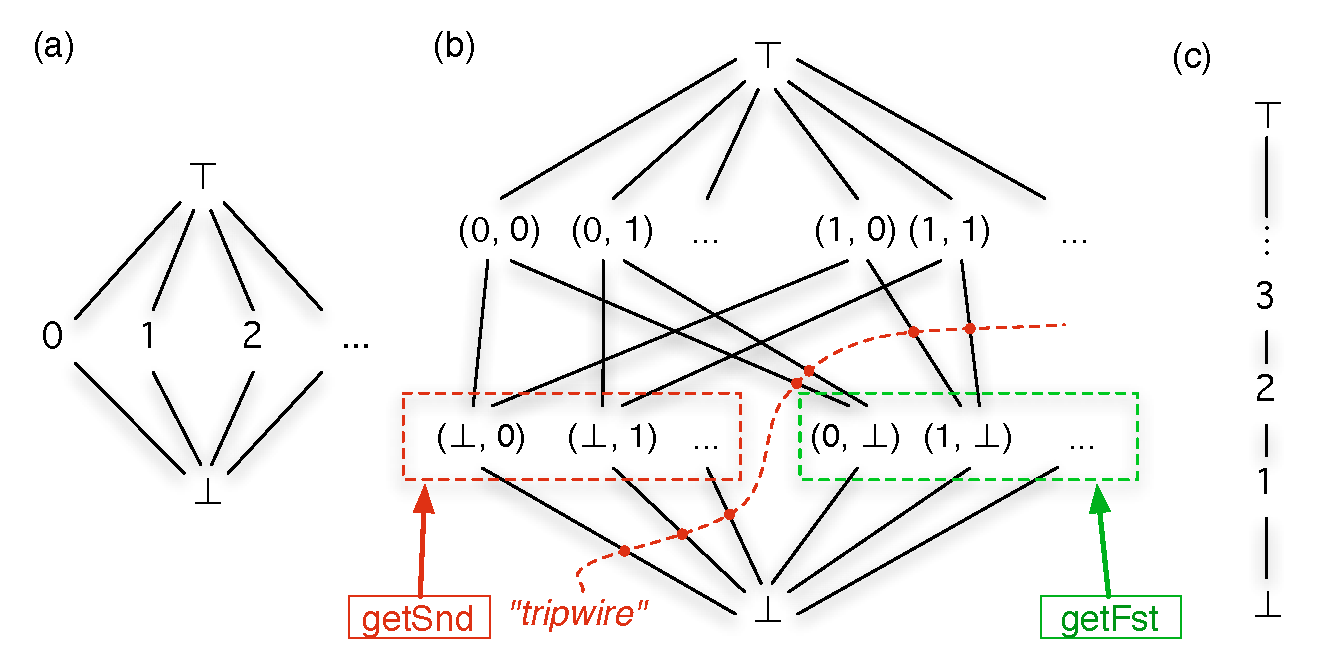
\includegraphics[width=5in]{chapter2/figures/ExampleLattices2.pdf} 
  \caption{Example lattices: (a) IVar containing a natural number; (b)
    pair of natural-number-valued IVars; (c) positive integers ordered
    by $\leq$ (see Section~\ref{subsection:lvars-fixme}\TODO{Add
      forward reference to to where I talk about generalizing put to
      bump.}).  Subfigure (b) is annotated with example threshold sets
    that would correspond to a blocking read of the first or second
    element of the pair (see
    Sections~\ref{subsection:lvars-communication-primitives} and
    \ref{subsection:lvars-programming-with-put-and-get}).  Any state
    transition crossing the ``tripwire'' for \termfont{getSnd} causes
    it to unblock and return a result.}
    \label{f:lvars-example-lattices}
\end{figure}

Figure~\ref{f:lvars-example-lattices} gives three examples of lattices
for common data structures.  The simplest example of a useful
lattice is one that represents the states that a a single-assignment
variable (that is, an IVar) can take on.  A natural-number-valued
IVar, for instance, has a state space corresponding to the lattice in
Figure~\ref{f:lvars-example-lattices}(a), that is,
\begin{displaymath}
  D = (\lbrace \top, \bot \rbrace \cup \mathbb{N}, \userleq), 
\end{displaymath}
where the partial order $\userleq$ is defined by setting $\bot
\userleq d \userleq \top$ and $d \userleq d$ for all $d \in D$.  This
is a lattice of height three and infinite width, where the naturals
are arranged horizontally.  After the initial write of some $n \in
\mathbb{N}$, any further conflicting writes would push the state of
the IVar to $\top$ (an error).  For instance, if one thread writes $2$
and another writes $1$ to an IVar (in arbitrary order), the second of
the two writes would result in an error because $2 \sqcup 1 = \top$.

In the lattice of Figure~\ref{f:lvars-example-lattices}(c), on the
other hand, the $\top$ state is unreachable, because the least upper
bound of any two writes is just the maximum of the two.  For instance,
if one thread writes $2$ and another writes $1$, the resulting state
will be $2$, since $2 \sqcup 1 = 2$.  Here, the unreachability of
$\top$ models the fact that no conflicting updates can occur to the
LVar.

\subsection{Stores}\label{subsection:lvars-stores}

During the evaluation of a $\lambdaLVar$ program, a \emph{store} $S$
keeps track of the states of LVars.  Each LVar is represented by a
binding from a location $l$, drawn from a set $\Loc$, to its state,
which is some element $d \in D$.  Although each LVar in a program has
its own state, the states of all the LVars are drawn from the same
lattice $D$.  We can do this with no loss of generality because
lattices corresponding to different types of LVars could always be
unioned into a single lattice (with shared $\top$ and $\bot$
elements).\footnote{Alternatively, in a typed formulation of
  $\lambdaLVar$, the type of an LVar might determine the lattice of
  its states.}

\begin{definition}\label{def:lvars-store}
A \emph{store} is either a finite partial mapping $S : \Loc \fmap
(D-\lbrace \top \rbrace)$, or the distinguished element $\topS$.
\end{definition}

I use the notation $\extSRaw{S}{l}{d}$ to denote extending $S$ with a
binding from $l$ to $d$.  If $l \in \dom{S}$, then $\extSRaw{S}{l}{d}$
denotes an update to the existing binding for $l$, rather than an
extension.  I also denote a store by explicitly writing out all its
bindings, using the notation $\store{\storebindingRaw{l_1}{d_1},
  \dots, \storebindingRaw{l_n}{d_n}}$.  The state space of stores
forms a bounded join-semilattice augmented with a greatest element,
just as $D$ does, with the empty store $\bot_S$ as its least element
and $\topS$ as its greatest element.  It is straightforward to lift
the $\userleq$ and $\sqcup$ operations defined on elements of $D$ to
the level of stores:

\LVarsDefLeqStore

\LVarsDefLubStore

By Definition~\ref{def:lvars-lubstore}, if $\userlub{d_1}{d_2} =
\top$, then
$\lubstore{\store{\storebindingRaw{l}{d_1}}}{\store{\storebindingRaw{l}{d_2}}}
= \topS$.  Notice that a store containing a binding
$\storebindingRaw{l}{\top}$ can never arise during the execution of a
$\lambdaLVar$ program, because (as I will show in
Section~\ref{s:lvars-lambdalvar}) an attempted write that would take
the state of $l$ to $\top$ would raise an error before the write can
occur.

\subsection{Communication Primitives}\label{subsection:lvars-communication-primitives}

The @new@, @put@, and @get@ operations create, write to, and read
from LVars, respectively. The interface is similar to that presented
by mutable references:

\begin{itemize}
\item @new@ extends the store with a binding for a new LVar whose
  initial state is $\bot$, and returns the location $l$ of that LVar
  (\ie, a pointer to the LVar).
\item @put@ takes a pointer to an LVar and a singleton set containing
  a new state and updates the LVar's state to the \emph{least upper
    bound} of the current state and the new state, potentially pushing
  the state of the LVar upward in the lattice.  Any update that would
  take the state of an LVar to $\top$ results in an error.
\item @get@ performs a blocking ``threshold'' read that allows
  limited observations of the state of an LVar.  It takes a pointer to
  an LVar and a \emph{threshold set} $Q$, which is a non-empty subset
  of $D$ that is \emph{pairwise incompatible}, meaning that the lub of
  any two distinct elements in $Q$ is $\top$.  If the LVar's state $d$
  in the lattice is \emph{at or above} some $d' \in Q$, the @get@
  operation unblocks and returns the singleton set $\lbrace d'
  \rbrace$.  Note that $d'$ is a unique element of $Q$, for if there
  is another $d'' \neq d'$ in the threshold set such that $d''
  \userleq d$, it would follow that $d' \sqcup d'' \userleq d \neq
  \top$, which contradicts the requirement that $Q$ be pairwise
  incompatible.
\end{itemize}

The intuition behind @get@ is that it specifies a subset of the
lattice that is ``horizontal'': no two elements in the threshold set
can be above or below one another.  Intuitively, each element in the
threshold set is an ``alarm'' that detects the activation of itself or
any state above it.  One way of visualizing the threshold set for a
@get@ operation is as a subset of edges in the lattice that, if
crossed, set off the corresponding alarm.  Together these edges form a
``tripwire''.  Figure~\ref{f:lvars-example-lattices}(b) shows what the
``tripwire'' looks like for an example @get@ operation.  The
threshold set $\stateset{(\bot, 0), (\bot, 1), ...}$ (or a subset
thereof) would pass the incompatibility test, as would the threshold
set $\stateset{(0, \bot), (1, \bot), ...}$ (or a subset thereof), but
a combination of the two would not pass.

The requirement that the elements of a threshold set be pairwise
incompatible limits the expressivity of threshold sets.  In fact, it
is a stronger requirement than we need to ensure determinism.  Later
on, in Section~\ref{s:lvars-generalized-threshold-sets}, I will
explain how to generalize the definition of a threshold set to make
more programs expressible.  For now, I will proceed with the simpler
definition above.

\subsection{Monotonic Store Growth and Determinism}\label{subsection:lvars-monotonic-store-growth}

In IVar-based languages, a store can only change in one of two ways: a
new, empty location (pointing to $\bot$) is created, or a previously
$\bot$ binding is permanently updated to a meaningful value.  It is
therefore straightforward in such languages to define an ordering on
stores and establish determinism based on the fact that stores grow
monotonically with respect to the ordering. For instance,
\emph{Featherweight CnC}~\cite{CnC}, a single-assignment imperative
calculus that models the Intel Concurrent Collections (CnC) system,
defines ordering on stores as follows:\footnote{A minor difference
  between $\lambdaLVar$ and Featherweight CnC is that, n Featherweight
  CnC, no store location is explicitly bound to $\bot$.  Instead, if
  $l \notin \dom{S}$, then $l$ is defined to point to $\bot$.}

\LVarsDefLeqStoreCnC

Our Definition~\ref{def:lvars-leqstore} is reminiscent of
Definition~\ref{def:lvars-leqstore-cnc}, but
Definition~\ref{def:lvars-leqstore-cnc} requires that $S(l)$ and
$S'(l)$ be \emph{equal}, instead of our weaker requirement that $S(l)
\userleq S'(l)$ according to the user-provided partial order
$\userleq$.  In $\lambdaLVar$, stores may grow by updating existing
bindings via repeated @put@s, so
Definition~\ref{def:lvars-leqstore-cnc} would be too strong; for
instance, if $\bot \userlt d_1 \userleq d_2$ for distinct $d_1, d_2
\in D$, the relationship
$\leqstore{\store{\storebinding{l}{d_1}}}{\store{\storebinding{l}{d_2}}}$
holds under Definition~\ref{def:lvars-leqstore}, but would not hold
under Definition~\ref{def:lvars-leqstore-cnc}.  That is, in
$\lambdaLVar$ an LVar could take on the state $d_1$ followed by $d_2$,
which would not be possible in Featherweight CnC.

I establish in Section~\ref{s:lvars-proof} that $\lambdaLVar$ remains
deterministic despite the relatively weak $\leqstore{}{}$ relation
given in Definition~\ref{def:lvars-leqstore}.  The keys to maintaining
determinism are the blocking semantics of the @get@ operation and the
fact that it allows only \emph{limited} observations of the state of
an LVar.
